%\documentclass{article}
\documentclass[letterpaper, 10 pt, conference]{ieeeconf}
\usepackage[utf8]{inputenc}
\usepackage{url}
\usepackage{hyperref}
%\usepackage[showframe=true]{geometry}
%\usepackage[usenames,table]{xcolor}
%\usepackage{titlepic} 
\usepackage{graphicx}
\usepackage{subfigure}
\usepackage[font=small]{caption}
\usepackage{amssymb,amsmath,amsthm}
\usepackage{capt-of}
\usepackage{textcomp}
%\usepackage{caption}
%\usepackage{titling}
\usepackage{algorithm2e}
\usepackage{amsmath,lipsum}
\usepackage{siunitx} % Provides the \SI{}{} and \si{} command for typesetting SI units
\usepackage{graphicx} % Required for the inclusion of images
\usepackage{mathtools}
\usepackage{xcolor}
\usepackage{amssymb}
\usepackage{sidecap}
\usepackage{amssymb}
\usepackage{array,multirow,graphicx}
\usepackage{booktabs}
\usepackage{rotating}

\newcommand\numberthis{\addtocounter{equation}{1}\tag{\theequation}}

%\overrideIEEEmargins

\title{
\includegraphics[scale = 0.05]{img/logo_unige.jpeg} \\ Energy saving room scheduling system for smart hotels}
\author{Ernesto Denicia, Emanuele Sansebastiano, Rocco Caravelli}
%\date{July 2016}

% geometry and page settings
%\geometry{includehead,includefoot}
%\geometry{inner=2cm,outer=2cm,top=2cm,bottom=2cm}
\parskip = 3pt
\parindent = 0pt
%\\ make a blannk line where they r located

\newcommand\T{\rule{0pt}{2.6ex}}% aggiungi spazio sopra riga di tabella

\DeclareMathOperator{\Ker}{Ker}
\DeclareMathOperator{\spn}{span}
\DeclareMathOperator{\sinc}{sinc}

% links colors
\hypersetup{
	colorlinks,
	%	linkcolor={orange},
	%	citecolor={black},
	%	urlcolor={blue}
}



\begin{document}		

\maketitle

\small

\section{Abstract}
Energy management is one of the most important aspects treated in Engineering and sciences. Either a path planning problem or an energy harvesting field of wind turbines, the necessity to ensure optimality is always present when competitivity is desired. Optimisation at the service of Engineering is a broad field of development and deals with a very dynamic set of applications that can be present even in the normal life.

While technology is improving with time, new intelligence layers are being added to existing systems in order to make them reactive to predefined constraints \cite{intelligent_decisions}. Optimisation problems that were before only tangible for those having to do directly with the development of a product are becoming every day more popular and widely used by normal users.

Hotels and other accommodation providers deal with the problem of assigning booking requests in an optimum way. The majority of homologous systems attempt to forecast the energy consumption of the analysed buildings or to monitor it and propose alternative solutions to decrease it \cite{university}. Others already go a step further in proposing systems that optimise tenants' comfort or energy consumption reduction by means of complex techniques like reinforcement learning \cite{reinf_learn} while at the same time adapting them to the usage pattern of the user.

While approaching in the same manner the multi objective problem of assigning the rooms to the guests in the most profitable way, this work deals also with the construction of an agent with an extra intelligence layer capable of choosing assignment sequences that ensure optimality in the sense of energy consumption. This framework can be envisioned as part of a smart building environment and chapter \ref{intro} introduces formally the problem formulation that motivates its creation. Chapter \ref{state_art} analyses further the actual situation of the development field and gives an insight on the profitability of such a system in the actual environment. Chapters \ref{development} and \ref{campaign} describe more deeply the development and validation strategies adopted and finally, chapter \ref{results} concludes on the topic and provides an outlook with possible future improvements.

\section{Introduction and proposal} \label{intro}
Even though energy consumption is penalised by governmental bodies with norms like DPR 412/1993 \cite{normDPR}, it is also in the interests of hotel managers to ensure a lower energy consumption as it generates a more profitable situation for them. One could naively think that such a system would only be profitable for winter season, while in reality, in summer the problem happens in the same form as temperature regulation is needed. As an initial proposal, it is interesting to look for solutions that ensure profit maximisation as a first priority and then looks in the feasible set of assignments for those being energetically optimal.

In this context, the next assumptions were taken
\begin{enumerate}
	\item Assume the existence of differed heat sources in every room of the building. This widens the research field and helps understand better the optimisation problem due to the variety in degrees of freedom.
	\item Common areas like corridors or lounges should be heated up whenever new clients arrive. 
	\item Without losing generality, assignment of a room implies its direct heating given that its coupling relations with other rooms are to be considered.
	\item A model predictive approach is to be used in order to broaden the degree of action of controls on the building to be considered.
\end{enumerate}

An example that motivates this direction of research can be seen in Fig.~\ref{figTemper_onoff}. A lumped-parameter model of a hotel consisting of three floors and more than 80 rooms was designed and tested. A regular ON-OFF control strategy was adopted for its simulation, given that it is the common approach adopted for temperature management in the real life. As seen, while the first and third floor  are heated up, the second floor finds itself already at the optimal temperature value, for which assigning a new booking request to any of the rooms in the middle would be a more intelligent solution from an incipient energy optimising approach.

\begin{figure}[htbp]
	\centering
	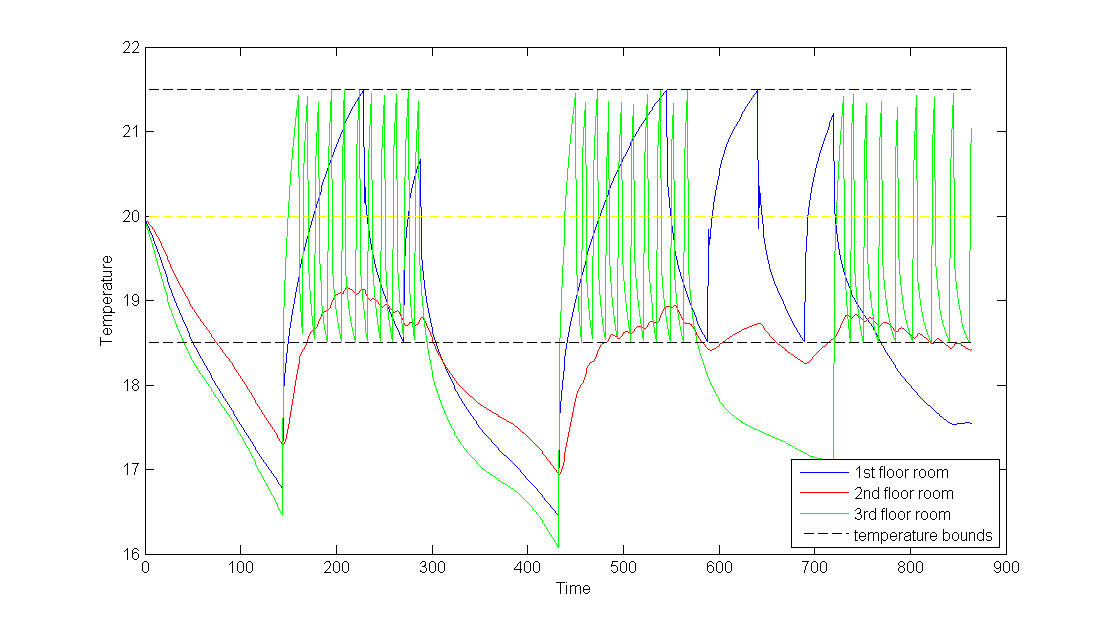
\includegraphics[width=0.45\textwidth, height=0.22\textwidth]{img/temperature_anal.png}
	\caption{\textit{Temperature of three rooms located one over the other having various customers along 6 days.}}
	\label{figTemper_onoff}
\end{figure}

Finally, it is important to say that the energetically optimal solutions are not necessarily predictable, and are expected to be dependent on several preconditions, among which the isolating performance of the hotel can be of interest. One attempts, however to exploit the adjacency relations of the rooms, the existence of natural heating sources like the sun radiation and a good estimation of the outer temperature to enrich a model in order to be able to forecast the energy consumption and to pick the best solution.




%\section{Robotic application}


\section{State of the art}
%\subsection{Analysis of the market}
This analysis is performed in two important directions: the commercial and the research ones. In the commercial field, only 20\% of the hotel managers are used to looking for consistent demand statistics and use them actively for demand forecasting and profit management operations. The majority consider only the tourist information provided by specialized agencies instead of looking at past booking data to conclude on this. The existence of a software managing the whole bookings system is a common characteristic of many hotels. 

The algorithms existing in the market either in specialized softwares or open source solvers, over all those being used in Italy require the owner of the building to load the prices and priorities of the rooms for making its decisions. These softwares, however, tackle mostly the point of revenue management optimisation (offer campaigns and calculation of optimal room prices) but do not direct its resources in determining the optimal booking out of a given booking request situation. Until today, random assignments and first book - first take policies have been implemented in order to achieve not only a profit but also convenient client satisfaction.

If a few quantity of the software market is directed to optimising the booking, one can imply that even a smaller one attempts to optimize the objective from different perspectives. A smart agent in this sense would be an attractive proposal for optimising decreasing the energy consumption while maintaining the revenue at a maximum level. As commented afterwards, the problem of client satisfaction and personalized use forecasting while ensuring feasibility on the final solutions determines also an important developmental direction and a allows to generate an intelligent framework capable of deciding on the assignment based on a more objective complexity level \cite{grids}.

In the field of research, many works have attempted to manage the consumption of energy from a centralized point of view, in which small clients subscribe to a bigger entity in order to decrease the consumption by means of a closed communication mechanism \cite{central}. Domotics is an area dedicated to the automation of environments and to the increasing of their receptiveness to human beings in order to perform tasks more optimally. One of the most salient topics in the present has been that of providing different frameworks with the awareness of energy consumption and with it generate even communication patterns that ensure optimality in request reception (e.g. turn off the lights and turn them on again)\cite{web}.

A framework like the one proposed in this work would therefore:
\begin{enumerate}
	\item Represent a good opportunity to compete against softwares using other decision techniques.
	\item Ensure the capacity of solving multi objective problems.
	\item In both dimensions it implies improvements with respect to existing techniques
\end{enumerate}


%\subsection{Criteria used}
%???? \label{state_art}%done
 
\section{Previous heat and control analysis}
In order to analyse the heat fluxes governing the heat transmission of a building there are two ways to proceed: taking blueprints of the building and, knowing all the material properties, making a heat analysis of every room, or taking the temperature of every room and identify the parameters to know the behave of heat fluxes. Because both approaches lead to the solution, we decided to make two independent previous analysis. \\
Each procedure is based on the equivalence having on the left side the summation of heat fluxes at a specific time instant and on the right side the variation of the internal energy from an instant to the following one:
$$q_{tot_{t}} = \Sigma q_{k_{t}} + \Sigma q_{h_{t}} + \Sigma q_{vent_{t}} + \Sigma q_{sun_{t}} + q_{pump_{t}}$$
$$q_{tot_{t}} = \rho V c_{p} \frac{d T}{d t}$$
Where:

$q_{k}$ is the thermal convection; \\
$q_{h}$ is the thermal conduction; \\
$q_{vent}$ is the ventilation flux according to the norm UNI/TS 11300; \\
$q_{sun}$ is the sun radiation took from weather forecast; \\
$q_{pump}$ is the heat flux coming from the heat pump (if activated); \\
$\rho V c_{p} \frac{d T}{d t}$ is the time derivative of the internal energy.

\subsection{Blueprint analysis strategy}
Since the used scenarios must be realistic we planned three kind of room according with their price and structure ($25$ $m^2$, $50$ $m^2$, $75$ $m^2$) and the same amount of customer kinds.
Every wall is made by common bricks (density: $2000$ $\frac{kg}{m^3}$; heat capacity: $0.9$ $\frac{kJ}{kg K}$; thermal conduction: $8 e^{-4}$ $\frac{kJ}{s m K}$); the exterior wall thickness is $0.4$ $m$, while the interior one is $0.1$ $m$. Every room have at least a window and one door on the corridor. The windows are made by common glass (density: $2400$ $\frac{kg}{m^3}$; heat capacity: $0.84$ $\frac{kJ}{kg K}$; thermal conduction: $9.6 e^{-4}$ $\frac{kJ}{s m K}$), and its thickness is $0.04$ $m$, while the doors are assumed to be like the interior wall for their heat behaviour. To run these initial set of experiments we decided to use real heat pumps (any other kind of heat source do not change the result) taken by the commercial catalogue Daikin Industries, in particular we used the heat pump called 'FTXZ35N'.

Due to the fact computer cannot handle continuous domain, the heat transfer equation must be discrete:
$$q_{tot_{t}} = \rho V c_{p} \frac{d T}{d t} \hspace{5mm} --> \hspace{5mm} \frac{q_{tot_{t}}}{\rho V c_{p}} = \frac{T_{t+1} - T_{t}}{time \\ gap}$$
Then, we can rewrite the equation:
$$K_{i,j} (T_{i,t} - T_{j,t}) = \frac{C_{i}}{time \\ gap} (T_{i,t+1} - T_{i,t})$$
Where:

$K_{i,j}$ is the heat transfer coefficient from the room j to i; \\
$C_{i,j}$ is the capacitance of the room i;

\subsection{System identification strategy}
The practise requires the temperature of the air of each room at each instant of the analysis   



E-plus

bla bla

\subsection{P control vs. ON/OFF control}


map of the hotel

different curves for the temperature depending on floors

gap-time

Assumptions on the hotel (temperature in - out, sun)




\subsection{Decision and control layers}

For this work, two layers of intelligence are provided. One dealing with the revenue maximisation problem, which returns the assignment of clients to the rooms according to the booking characteristics and the commercial description of the rooms involved in the building. The second layer represents a lower level optimal control problem that ensures minimal energy consumption for an imposed maximum revenue and which depends on the topology and adjacency relationships within the rooms, exterior and ground.

With consideration of the sets:

\begin{align*}
& d \in D=\{0, 1, ...n_d\}\\
& r \in R=\{0, 1...n_c, n_c+1 ... n_s ... n_r \}=\bigcup\{R_c,R_s\}\\
& R_d \subseteq R\\
& R_{dn} = R_d \bigcup {\gamma} \\
& d \in D_d \subseteq D\textbackslash d\\
& t \in T_1=\{1...N\}\\
& t \in T_2=\{1...N+1\}\numberthis
\end{align*}

described by booking requests set $D$, $R$ available $n_r$ rooms in building, out of which there are $n_c$ client rooms and $n_s$ service rooms or common areas (corridors and lounges), $R_d$ compatible rooms to request $d$ (in the case of considering the dummy node $\gamma$, one considers $R_{dn}$), the time sets $T_1$ and $T_2$ for revenue and energy consumption optimisation problems respectively and $D_d$ competing requests of request $d$.

The corresponding constants defined for this step of development are:
\begin{align*}
& T_{sp} = 20\\
& \hat{T}_{i,1}\\
& q^S_{i,t} \text{, } T_{e,t}\\
& K_{i,j} \text{ and } c_{i} \forall i,j\mid i,j\in R \text{, } i\sim j \numberthis
\end{align*}

where $T_{sp}$ determines the temperature setpoint to be reached when a room is selected. The initial temperature states of each room are imposed to be $\hat{T}_{i,1}$. The exogenous inputs $q^S_{i,t}$ and $T_{e,t}$ correspond to the solar radiation through the windows of each room differentiated according to its position on the Earth and the external temperatures measured at every sample. Finally, the transmittance and capacitance parameters $K_{i,j}$ and $c_i$ obtained either through initial theoretical estimate or  parameter identification routines.

With this information, the decision variables used for the solution of both optimisation problems are:
\begin{align*}
& x_{d,r}\in\mathbb{B} \text{ }\forall d\in D \text{ and } r\in{Rd}\bigcup \{\gamma\}\\
& z_{i,t}\in\mathbb{B} \text{ }\forall i\in{Rd} \text{ and }t\in T\\
& T_{i,t}\in\mathbb{C} \text{ }\forall i\in{Rd} \text{ and }t\in T\\
& u_{i,t}\in\mathbb{C} \text{ }\forall i\in{Rd} \text{ and }t\in T\numberthis
\end{align*}

The complete optimisation problem with emphasis on its linear multi objective nature is shown in Eq.~\ref{eq:opt_multi}.

 \begin{flalign*}
 &\begin{array}{rlclcl}
 \displaystyle Y^*=\max_{x_{d,r}} & \multicolumn{3}{l}{\sum_{d\in D}\sum_{r\in R_d}Y_{d,r}x_{d,r}} \\
 \textrm{s.t.} & \sum_{r\in R_{dn}}x_{d,r}=1 \text{ }\forall d\in D \\
 & x_{d,r}+x_{k,r}\leq 1 \text{ } \forall d\in D\text{, }\forall k\in D_d\\
 & \text{ and } \forall r\in R_d\cap R_k
 \end{array}\\
  &\begin{array}{rlclcl}
  \displaystyle E^*=\min_{x_{d,r}} & \multicolumn{3}{l}{\sum_{t\in T}\sum_{i\in R}u_{i,t}} \\
  \textrm{s.t.} & \sum_{r\in R_{dn}}x_{d,r}=1 \text{ }\forall d\in D \\
  & x_{d,r}+x_{k,r}\leq 1 \text{ } \forall d\in D\text{, }\forall k\in D_d\\
  & \text{ and } \forall r\in R_d\cap R_k\\
  & z_{i,t} = \sum_{\substack{d\in D\\t_d^{in}\leq t \leq t_d^{out}}} x_{d,r} \text{ } \forall r\in R \text{, }\\
  &\forall t\in{T_1}\\ 
  & \hat{T}_{i,t+1}=\frac{1}{c_i}(\sum_{i\sim j\bigcup e}(\hat{T}_{i,t}-\hat{T}_{j,t})+\\
  & K_{u}u_{i,t}+q^S_{i,t}+\hat{T}_{i,t})\\
  & T_{i,1} = \hat{T}_{i,1}\\
  & u_{i,t}\geq 0\\
  & u_{i,t}\geq z_{i,t}(T_{sp}-T_{i,t})\\
  & z_{j,t} \geq \wedge z_{k,t} \text{ }\forall j\in{R_{s}} \text{ and }k\sim j\\
  & Y_{t}\geq Y^*
  \end{array}\\
  & \numberthis
 \label{eq:opt_multi}
 \end{flalign*}
 
 The aim of this multiobjective problem is that of generating optimal energetically performing assignments once the revenue was maximised. With this a clear differentiation between actual solvers in the market and this scheduling system can be highlighted. For the development of this task, the work is divided into the next steps:
 \begin{enumerate}
 	\item Solution of the revenue maximisation assignment problem (upper bound on revenue).
 	\item Generation of additional revenue-wise optimal solutions 
 	\item Determination of the energy consumption of each of the obtained solutions. (Energy efficiency estimation).
 	\item Solution of the energy consumption minimisation problem (energetical lower bound on maximal revenue solution).
 \end{enumerate}
 
 Notice than the profit is redefined to be depending on the kind of assignments $x_{d,r}$ performed instead of on attempting only to maximize income, which is also something that many easy solvers do. For this, six levels of profit were proposed, each for the compatible assignment of three levels of clients to three levels of rooms and accordingly to Table~\ref{tab:profits}.
 \begin{table}[htbp]
 	\centering
 	\caption{Levels of profits used as a marketing strategy for this work}
 	\begin{tabular}{cr|ccc}
 		\toprule
 		\multicolumn{2}{c|}{\multirow{2}[0]{*}{Request}} & \multicolumn{3}{c}{Room type} \\
 		\multicolumn{2}{c|}{} & Low  & Medium & High \\ 
 		\midrule
 		\multirow{2}[0]{*}{} & Low &   9   &   7    & 2 \\
 		& Medium &   0    &   22    &  17\\
 		& High &0 & 0& 72\\
 		\bottomrule
 	\end{tabular}%
 	\label{tab:profits}%
 \end{table}%
 
 The profit was proposed in representative costs, not related to the real world and chosen with the proposal of a desired probability distribution to allow for approachability into a more real scenario. Notice that this profit definition does not suppress the possibility of assignment of high level rooms to low level requests, for which it is also possible to include an intelligent offer for the clients to ensure their pleasure as much as these profit values are tuned. As an example, one could consider the hotel in Fig.~\ref{fig:smallhotel} with rooms 5 and 6 categorised as a high level rooms and rooms 9 and 10 with the biggest amount of solar irradiation (therefore energetically less demanding, at least in a direct sense).
 
    \begin{figure}[thpb]
    	\centering
    	\framebox{\parbox{3in}{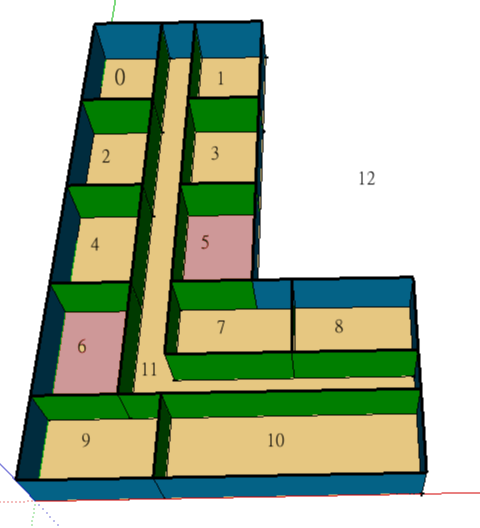
\includegraphics[width=77mm]{img/small_hotel.png}}}
    	%\includegraphics[scale=1.0]{figurefile}
    	\caption{Forward simulation of the system after parameter identification.}
    	\label{fig:smallhotel}
    \end{figure} 
    
After running the framework, one can find, among the several solutions, that by ensuring the optimum revenue value, it is possible to get energetically less demanding solutions preferring to start assigning rooms near rooms 9 and 10 than farther away. Notice that for this case, the fact that one room is occupied implies that the temperature of the central corridor (11) is also set to $T_{sp}$ so that it might become more difficult to give a direct interpretation of the solutions. Nevertheless, the optimisation framework approach corresponds to a software robot capable of deciding for the owner of the building which rooms to assign by protecting the revenue, ensuring least energy consumption and learning the real parameters of the system for further proposals.

\section{Data used and experimental campaign} \label{campaign}
\subsection{Data}
As said before, this work attempts to find optimal solutions in means of revenue and energy on two kinds of hotel. The first case corresponds to an easily found small scale hotel with one floor and with 20\% of its rooms only dedicated to high level requests. In the scale commented before, six rooms where imposed as low level, 3 as middle range and 1 as high level. The bigger hotel, on the other hand counts with 23 rooms (15 low , 6 medium , 2 high), with 7 of them located on the first floor, and 8 on the other two. This information is necessary for planning the demand.

The optimal analysis should take place every time there is a new request, introducing the already occupied rooms as constraints. For analysis purposes, however, an optimisation horizon of two weeks was proposed. Fig.~\ref{figDemand_stat} shows the distribution used for planning the demand and based on information provided by a marketing analysis from ISTAT \cite{istat} in Liguria. Also, the weather parameters were taken from a Genova weather file, including those of the exterior temperature, ground temperature and solar radiation. \cite{weather}

\begin{figure}[htbp]
	\centering
	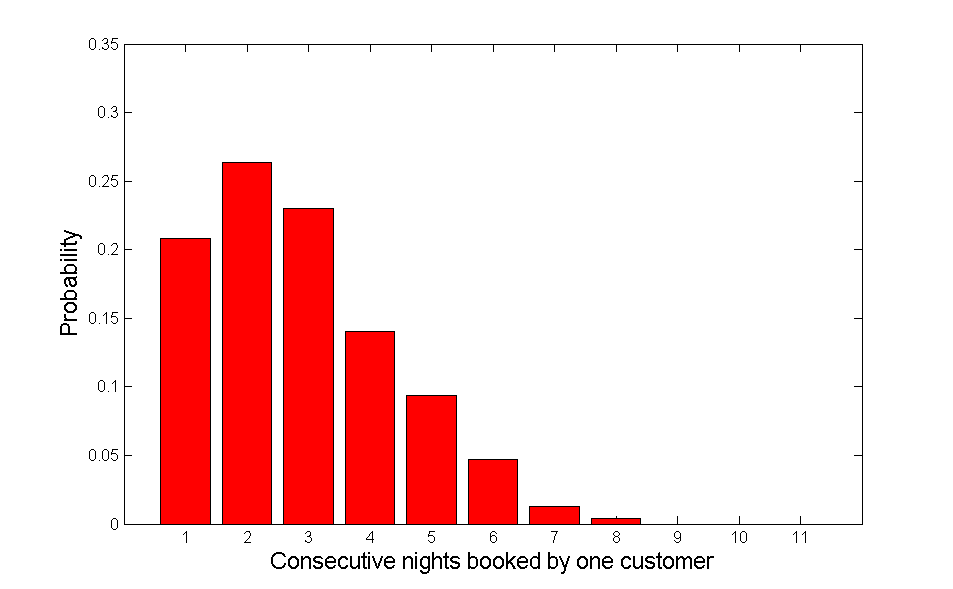
\includegraphics[width=0.45\textwidth, height=0.22\textwidth]{img/Booking_probability1.png}
	\caption{\textit{Statistical distribution of the consecutive number of night asked by a customer.}}
	\label{figDemand_stat}
\end{figure}

As explained before, the revenue is not just dependent on the price of the room, but also on the maintenance costs of the room which is about one tenth of the room's price (1, 3, 8 [$\frac{money}{night}]$). Finally, according to the formulation, a compatible costumer for a room can stay in a upper quality room paying the same price as offered during the booking request. So, since the revenue is the difference between price and maintenance cost of a room, the hotel can get 6 possible revenues according the combinations seen in Table~\ref{tab:profits}.

\subsection{Experimental campaign}
A non-dimensional index was proposed in order to evaluate the performance of the scheduling system against that of common assignment approaches: The Relative Percent Deviation- RPD.
$$RPD = \frac{|X_{o} - X_{r}|}{X_{o}}\times 100$$
Where:
$X_{o}$ is a characteristic measure of the energy obtained by using any assignment ensuring maximum profit.
$X_{r}$ corresponds to the optimal energy solution with maximum revenue as constraint.

An important variable taken into consideration is the percentage occupancy of the hotel. If it were 100\% occupied, there would not be any reason to optimize the assignment of customers. Characteristic rates of approximately 30\%, 50\% and 65\%. Because the demand is generated before optimizing the revenue and some of the requests can be rejected during this step, some extra demand was added in order to remain about the above mentioned values. 

Notice that the optimal energy consumption solution is not compared against any possible assignment given by any solver with non optimizing characteristics but rather against the heuristic solution of the solver used for optimisation (Gurobi). Moreover, to ensure robustness of the analysis form the statistical point of view, 10 instances per occupancy rate were generated for each of the two topologies and the optimisation process was run on five several solutions per instance and averaged. The RPD[\%] can be then computed out of these comparison quantities.



  






\section{Results and conclusion} \label{results}
%\subsection{Results}
Table \ref{Table_RPD} confirms the fact that for this optimisation run, energy is saved. 

\begin{table}[htbp]
	\centering
	\caption{Relative percentage difference}
	\label{Table_RPD}
	\begin{tabular}{lllll}
		Occupancy     & 30\%  & 50\% & 65\%  \\
		Hotel 1-floor & 5.68  & 8.88 & 4.27  \\
		Hotel 3-floor & 11.27 & 8.73 & 4.27  \\
	\end{tabular}
\end{table}

In general, the obtained results prove that an increasing revenue is ensured for lower occupancy rates. However, the small hotel (30\% occupancy rate) seems not to follow this expected behaviour. By analysing particular results, it was possible to propose possible causes to this event:
\begin{enumerate}
	\item In many of the cases, more than one overlapping high quality rooms were proposed. The small hotel counts only with one high quality room and therefore the degree of compatibility in different assignments potentially decreases. Maximum revenue can therefore only be obtained by reassigning low and medium level rooms.
	\item It was possible to notice that the solar radiation had an important effect on the dynamics of the system. Rooms facing the south side of the building are favoured with more solar radiation. For some cases, the energy consumption optimised assignment selected rooms near this location first, however the higher level rooms were located in unfavoured locations with respect to solar irradiation. This again constrained the capacity of assignation for which both energetic and revenue optimisation approaches were very similar in nature.
\end{enumerate}


\begin{thebibliography}{1}
	
	\bibitem{intelligent_decisions} Adhikari Animesh, Intelligent Decision Technologies - Volume Preprint, issue Preprint,  vol. Preprint, no. Preprint, pp. 1-12, 2014 
	
	\bibitem{normDPR} D.P.R. 26 agosto 1993, n. 412 {\em Pubblicato nella Gazz. Uff. 14 ottobre 1993, n. 242, S.O}
	
	\bibitem{normUNI} UNI/TS 11300 {\em Prestazioni energetiche degli edifici} 2014:
		
	\bibitem{daikin} Daikin {\em heat pumps catalogue} 2014
	
	\bibitem{istat} ISTAT {\em Annuario statistico italiano} 2013
	
	\bibitem{weather} EnergyPlus {\em https://energyplus.net/weather-location}
	
	\bibitem{reinf_learn} Fazenda, Pedro; Veeramachaneni, Kalyan; Lima, Pedro; O'Reilly, Una-May; Using reinforcement learning to optimize occupant comfort and energy usage in HVAC systems, Journal of Ambient Intelligence and Smart Environments, vol. 6, no. 6, pp. 675-690, 2014.
	
	\bibitem{university} Stavropoulos, Thanos G.;  Koutitas, George; Vrakas, Dimitris; et.al., A smart university platform for building energy monitoring and savings , Journal of Ambient Intelligence and Smart Environments, vol. 8, no. 3, pp. 301-323, 2016. 
	
	\bibitem{grids} Gajowniczek, Krzysztofa; Zabkowski, Tomasza; Short term electricity forecasting based on user behavior from individual smart meter data,  Journal of Intelligent \& Fuzzy Systems, vol. 30, no. 1, pp. 223-234, 2015
	
	\bibitem{storage} Botón-Fernández, Vicentea; Lozano-Tello, Adolfoa;  Pérez-Romero, Máximob; Romero-Cadaval, Enriqueb; Mining sequential patterns to efficiently manage Energy Storage Systems within smart home buildings, Journal of Ambient Intelligence and Smart Environments, vol. 8, no. 3, pp. 287-300, 2016.
	
	\bibitem{web} Kamilaris, Andreas; Pitsillides, Andreas ; Yiallouros, Michalis; Building energy-aware smart homes using web technologies, Journal of Ambient Intelligence and Smart Environments, vol. 5, no. 2, pp. 161-186, 2013.
	
	\bibitem{central} Botón-Fernández, Vicente; Lozano-Tello, Adolfo Pérez-Romero, Máximo Romero-Cadaval, Enrique, Mining sequential patterns to efficiently manage Energy Storage Systems within smart home buildings, Journal of Ambient Intelligence and Smart Environments, vol. 8, no. 3, pp. 287-300, 2016
	
\end{thebibliography}


%The robot used to collect the data is a Lego NXT robot equipped with a sensor developed at ECN. This robot is classified as a unicycle robot (2,0). The sensor bar is made of eight binary Reed sensors, which detects magnetic field. The detectors are spaced by 1 cm. The strip of sensors is located so that it is perpendicular to the x-axis of the robot, at a known position along $\textrm{X}_m$.
%The magnets are the beacons of the localization system. They are arranged as a squared array with a spacing of 55 mm.
%
%The robot also has two encoders, with a resolution of 360 dots per revolution.
%
%The localization system uses an EKF (Extended Kalman Filter).
%
%\section{First Lab}

In this first lab session, the use of extended Kalman filter for path estimation has been investigated. The complete Matlab files are provided in the folder \texttt{src/part1}.

\subsection{Discrete Evolution Model}\label{secDiscreteModel}

The model of the robot in continuous time can be expressed as\footnote{The value of $2L$ corresponds to the distance between the fixed wheels, represented in the Matlab files by the variable \texttt{trackGauge}.}:
$$\left[\begin{array}{c}
\dot{x} \\ \dot{y} \\ \dot{\theta}
\end{array}\right] =
\left[\begin{array}{c}
V\cos\theta \\ V\sin\theta \\ \omega
\end{array}\right]
\qquad\qquad
\left[\begin{array}{c}
V \\ \omega
\end{array}\right] =
\left[\begin{array}{cc}
\frac{r}{2} & \frac{r}{2} \\ \frac{r}{2L} & -\frac{r}{2L}
\end{array}\right] 
\left[\begin{array}{c}
\dot{q}_R \\ \dot{q}_L
\end{array}\right]
$$

Through a forward Euler discretization we can obtain the following:
$$\left[\begin{array}{c}
x_{k+1} \\ y_{k+1} \\ \theta_{k+1}
\end{array}\right] =
\left[\begin{array}{c}
x_k + U_{1,k}\cos\theta_k \\ y_k + U_{1,k}\sin\theta_k \\ \theta_k + U_{2,k}
\end{array}\right]
\qquad\qquad
\left[\begin{array}{c}
U_{1,k} \\ U_{2,k}
\end{array}\right] =
\left[\begin{array}{cc}
\frac{r}{2} & \frac{r}{2} \\ \frac{r}{2L} & -\frac{r}{2L}
\end{array}\right] 
\left[\begin{array}{c}
\Delta q_{R,k} \\ \Delta q_{L,k}
\end{array}\right]
$$
where $\Delta q_{R,k}$ represents the angle spanned by the right wheel within the time interval $\Delta t$ (i.e. $\Delta q_{R,k}=q_{R,k+1}-q_{R,k}$); the same works for $\Delta q_{L,k}$.

We implemented the model in the Matlab file called \texttt{EvolutionModel.m}, and we changed the script \texttt{ShowOdometry.m} so that it uses both our model and the default one (that has been renamed as \texttt{EvolutionModelDefault.p}). The correctness of our results is monitored by a matrix called \texttt{errX}, whose columns are defined as the difference given by the evolution of the new state obtained using the original \texttt{EvolutionModelDefault.p} and the state returned by our function. After the main loop of the script \texttt{ShowOdometry.m}, the error components are plotted in a figure. As expected, the result is that all the values are exactly zero, meaning that the model has been properly implemented.

Before proceeding, we had a look at the Cartesian speed of the robot. As shown in figure \ref{figSpeed} the estimation has some persistent oscillations. This is due to the not infinite resolution of the encoders, that introduce an error. The real linear speed is likely around $55\,\textrm{mm/s}$, while the angular one could be nearly zero.

\begin{figure}
	\centering
	\includegraphics[width=0.4\textwidth]{img/part1/odomVel.pdf}
	\caption{linear and angular speed estimated by odometry on the track \texttt{line1magnet}.}
	\label{figSpeed}
\end{figure}



\subsection{Extended Kalman Filter Equations}

The discrete time system that describes the evolution of robot's state has been already defined in the previous section:
$$\mathrm{X}_{k+1} =
\mathrm{X}_k + 
\begin{bmatrix} \cos\theta_k & 0\\ \sin\theta_k & 0\\ 0 & 1 \end{bmatrix}\mathrm{U}_k = 
f\left(\mathrm{X}_k, \mathrm{U}_k\right)
$$
In order to complete it, we need the following output equation:
$$ \mathrm{Y}_k =
\begin{bmatrix}
\cos\theta_k\left(x_m^\circ-x_k\right)+\sin\theta_k\left(y_m^\circ-y_k\right)\\
\cos\theta_k\left(y_m^\circ-y_k\right)-\sin\theta_k\left(x_m^\circ-x_k\right)
\end{bmatrix} =
g\left(\mathrm{X}_k\right)
$$
Where $\mathrm{Y}_k$ corresponds to the components of the distance between the detected magnet and the robot's origin (projected in robot's reference frame).

Since the system is not linear, the standard Kalman filter cannot be used; instead, we can evaluate the linear approximation of this system and estimate the path through an extended Kalman filter. The matrices that we need are the following:
\begin{flalign*}
A &= \frac{\partial f\left(\mathrm{X}_k, \mathrm{U}_k\right)}{\partial \mathrm{X}_k} = 
\begin{bmatrix}
1 & 0 & -U_{1,k}\sin\theta_k\\ 0 & 1 & U_{1,k}\cos\theta_k\\ 0 & 0 & 1
\end{bmatrix}
\\
B &= \frac{\partial f\left(\mathrm{X}_k, \mathrm{U}_k\right)}{\partial \mathrm{U}_k} =
\begin{bmatrix}
\cos\theta_k & 0 \\ \sin\theta_k & 0\\ 0 & 1
\end{bmatrix}
\\
C &= \frac{\partial g\left(\mathrm{X}_k\right)}{\partial \mathrm{X}_k} =
\begin{bmatrix}
-\cos\theta_k & -\sin\theta_k &
-\sin\theta_k\left(x_m^\circ-x_k\right)+\cos\theta_k\left(y_m^\circ-y_k\right)
\\
\sin\theta_k & -\cos\theta_k &
-\sin\theta_k\left(y_m^\circ-y_k\right)-\cos\theta_k\left(x_m^\circ-x_k\right)
\end{bmatrix}
\end{flalign*}






\subsection{Measurement Noise}

First of all, we set the covariance matrices all to zero. In such way, the estimation is assumed to be perfect, without noise.

In order to find the proper covariances, we reasoned about the factors that can corrupt the measurements. First of all, regarding the vertical component, i.e. \texttt{sigmaYmeasurement}, we assumed that a magnet could be located in any place between two sensors with uniform probability distribution, thus obtaining:
$$\sigma_{Ym} = \frac{\Delta Y}{\sqrt{12}} = \frac{10}{\sqrt{12}} $$
with $\Delta Y$ representing the spacing between two Reed receptors.

Regarding the value of \texttt{sigmaXmeasurement}, we considered two alternative methods for its calibration.

The first way is to set the scanning frequency to its maximum possible value (by setting \texttt{subSamplingFactor} to 1 in the file \texttt{RobotAndSensorDefinition.m}), make the robot follow a straight path (e.g. \texttt{line1magnet}) and check the region where a single magnet is detected more times consecutively. This allows to define an ``activation region'' for the sensors, namely $a_x$, that correspond to the interval where a sensor is able to detect the presence of a magnet. Referring to figure \ref{figHighSampling}, resulting from \texttt{line1magnet}, we found that a single magnet can be detected at most seven times.

\begin{figure}[htbp]
	\centering
	\hspace{\stretch{1}}
	\subfigure[Series of acquisitions from Reed sensors; each magnet is detected several times.\label{figHighSampling}]{\includegraphics[width=0.4\textwidth]{img/part1/samplingHighRate.pdf}}
	\hspace{\stretch{1}}
	\subfigure[Focus around a particular magnet. The activation region $a_x$ and the distance $d_x$ between two acquisitions are shown.\label{figHighSamplingZoom}]{\includegraphics[width=0.4\textwidth]{img/part1/samplingHighRateZoom.pdf}}
	\hspace{\stretch{1}}
	\caption{example of readings from the Reed sensors.}
\end{figure}

The distance between two consecutive scans is $d_x = 3\,\textrm{mm}$ (fig. \ref{figHighSamplingZoom}), and therefore we have that $a_x=18\textrm{mm}$. In addition, we must consider that the magnet could have activated the Reed sensors before the first measurement or after the last one. The estimated activation region has to be enlarged to $a_x+d_x=21\,\textrm{mm}$. We assumed that the magnet could be in any position of the activation region with the same probability, and therefore we could set \texttt{sigmaXmeasurement} to:
$$ \sigma_{Xm} = \frac{a_x+d_x}{\sqrt{12}} = \frac{21}{\sqrt{12}} $$

The previous method is based on the possibility of performing one test with a higher scanning sampling rate than the one normally used by the robot. Since this could be infeasible (because we simply cannot increase the sampling rate), a similar method to estimate measurement variance consists in repeating the same procedure with the standard sampling rate; in our case, we have to set \texttt{subSamplingFactor} to its original value, i.e. 4. Figure \ref{figLowSampling} shows the magnet detection in the test \texttt{diagonal45degrees}; due to the lower frequency, a magnet is detected at most 2 times, and therefore the values of $a_x$ and $d_x$ become the same: $12\,\textrm{mm}$ (fig. \ref{figLowSamplingZoom}). Therefore the position of a detected magnet can be, in the worst case, $12\,\textrm{mm}$ away from the activated Reed sensor. Assuming again a uniform probability distribution, it is possible to determine the standard deviation as:
$$ \sigma_{Xm} = \frac{a_x+d_x}{\sqrt{12}} = \frac{24}{\sqrt{12}} $$

\begin{figure}[htbp]
	\centering
	\hspace{\stretch{1}}
	\subfigure[Series of acquisitions from Reed sensors; each magnet is detected at most two times.\label{figLowSampling}]{\includegraphics[width=0.4\textwidth]{img/part1/samplingLowRate.pdf}}
	\hspace{\stretch{1}}
	\subfigure[Focus around a particular magnet. The activation region $a_x$ and the distance $d_x$ between two acquisitions here coincide.\label{figLowSamplingZoom}]{\includegraphics[width=0.4\textwidth]{img/part1/samplingLowRateZoom.pdf}}
	\hspace{\stretch{1}}
	\caption{example of readings from the Reed sensors.}
\end{figure}


%we guessed that any sensor can activate only within a \colorbox{pink}{restricted} area, $a_x$. In order to evaluate the length of this interval, we put the scanning frequency to the maximum possible (\texttt{subSamplingFactor = 1} in \texttt{RobotAndSensorDefinition.m}), and after one execution of \texttt{MagnetLoc.m} we obtained a the sequence of acquisitions shown in figure \ref{figMangetScanNoZoom}: one single magnet is detected several times, and therefore we can estimate the ``detectability range'' as the width of such sequence of readings (\ref{figMangetScanZoom}). We obtained $a_x=14\textrm{mm}$.
%
%\begin{figure}[htbp]
%	\centering
%	\hspace{\stretch{1}}
%	\subfigure[Series of acquisitions from Reed sensors; each magnet is detected several times.\label{figMangetScanNoZoom}]{\includegraphics[width=0.4\textwidth]{img/part1/figsamplinghigh.pdf}}
%	\hspace{\stretch{1}}
%	\subfigure[Focus around a particular magnet. The width $a_x$ is clearly shown and the additional uncertainty $f_x$ is reported referred to the case \texttt{subSamplingFactor=4}. \label{figMangetScanZoom}]{\includegraphics[width=0.4\textwidth]{img/part1/figsamplinghighzoom.pdf}}
%	\hspace{\stretch{1}}
%	\caption{example of readings from the Reed sensors.}
%\end{figure}
%
%In addition, there will be a further uncertainty coming from the readings frequency. One can imagine that, with an infinite frequency, the uncertainties will come from the value of $a_x$ only. However, since the readings have a finite frequency, the uncertainties will increase, and we can estimate them as the half of the distance between two sequential acquisitions. Once \texttt{subSamplingFactor} was reset to the initial value (i.e. 4), we found $f_x = 11\textrm{mm}$, that is the distance between two scans.

In conclusion, one can decides which method is more suitable. In general, the first one will be more precise, though not always feasible. Since it was possible to do so, we decided to set the value of \texttt{sigmaXmeasurement} to $\frac{21}{\sqrt{12}}$.



\subsection{Initial State Uncertainties}

Another parameter that has to be tuned is the variance of initial state. The error in the starting positioning is strictly related to user's imprecision in locating the robot in the proper location with the right orientation. We assumed that the positioning errors can be considered as Gaussian random variables with zero mean and standard deviations $\sigma_x = 5\,\textrm{mm}$, $\sigma_y = 5\,\textrm{mm}$ and $\sigma_\theta = 5^\circ$. With such values, initial errors will belong to the intervals $[-2\sigma,+2\sigma]$ with a probability of 95\%.





\subsection{Mahalanobis Threshold}

In order to choose a proper threshold for Mahalanobis distance, we used the Matlab function \texttt{chi2inv}, which has two parameters as input: the desired probability \texttt{P} of non-rejecting a good measure and the degrees of freedom \texttt{V} of our system. We used the two values \texttt{P=0.9} and \texttt{V=2} (\texttt{V} in this situation corresponds to the number of measurements that we have), thus obtaining the threshold $\sim\!4.6$.



\subsection{Tuning ``\texttt{sigmaWheels}''}\label{sectionSigmaWheel}

The last parameter that has to be tuned is \texttt{sigmaWheels}. To do so, we decided to run the program using the tracks named \texttt{oneloop} and \texttt{twoloops}; as criteria we chose the following:

\begin{enumerate}
	\item all the detected magnets must not be rejected;
	\item almost all neighbour magnets must be rejected;
	\item the initial and final position of the robot must be very similar.
\end{enumerate}

We used a dichotomic approach, starting from the value 1.0 as upper bound and 0 as lower bound. After some trials (some of them are shown in figure \ref{figSigmaTuning}; they have been performed on \texttt{twoloops}), the chosen value is \texttt{sigmaWheels = 0.1}, which ensures to reject the neighbours magnets and to keep the closest ones. In addition, initial and final positions are nearly equal (fig. \ref{figSigmaTuningPositions}).

\begin{figure}[htbp]
	\centering
	\hspace{\stretch{1}}
	\subfigure[$\sigma_W=1.0$]{\includegraphics[width=0.22\textwidth]{img/part1/mahaFail10.pdf}}
	\hspace{\stretch{1}}
	\subfigure[$\sigma_W=0.5$]{\includegraphics[width=0.22\textwidth]{img/part1/mahaFail05.pdf}}
	\hspace{\stretch{1}}
	\subfigure[$\sigma_W=0.2$]{\includegraphics[width=0.22\textwidth]{img/part1/mahaFail02.pdf}}
	\hspace{\stretch{1}}
	\subfigure[$\sigma_W=0.1$]{\includegraphics[width=0.22\textwidth]{img/part1/mahaFail01.pdf}}
	\hspace{\stretch{1}}
	\caption{tuning of $\sigma_W$ (\texttt{sigmaWheels}); the number of rejected neighbours magnet increases as $\sigma_W$ decreases. With $\sigma_W = 0.1$ we are able to reject all neighbours magnet while keeping the closest ones.}\label{figSigmaTuning}
\end{figure}

\begin{figure}[htbp]
	\centering
	\hspace{\stretch{1}}
	\subfigure[Track \texttt{oneloop}]{\includegraphics[width=0.22\textwidth]{img/part1/oneloop.pdf}}
	\hspace{\stretch{1}}
	\subfigure[Focus around initial an final positions]{\includegraphics[width=0.22\textwidth]{img/part1/oneloopFocus.pdf}}
	\hspace{\stretch{1}}
	\subfigure[Track \texttt{twoloops}]{\includegraphics[width=0.22\textwidth]{img/part1/twoloops.pdf}}
	\hspace{\stretch{1}}
	\subfigure[Focus around initial an final positions]{\includegraphics[width=0.22\textwidth]{img/part1/twoloopsFocus.pdf}}
	\hspace{\stretch{1}}
	\caption{estimated paths (odometry and KF) in the two tracks \texttt{oneloop} and \texttt{twoloops}. In both cases, the distance from initial to final position is around $3\,\textrm{mm}$, that could be due to human driver's imprecisions}\label{figSigmaTuningPositions}
\end{figure}

Finally, we tested this set of parameters with the other tracks, obtaining for all of them good estimations.

%
%\newpage
%
%\section{First Lab}

In this first lab session, the use of extended Kalman filter for path estimation has been investigated. The complete Matlab files are provided in the folder \texttt{src/part1}.

\subsection{Discrete Evolution Model}\label{secDiscreteModel}
%
\end{document}